\section{Test}

For at finde ud af hvordan der kan bestemmes en fornuftig grænseværdi, skal der findes ud af hvorledes magnitude for DTMF-frekvenserne ændrer sig under forskellige fysiske forhold - nærmere bestemt vinklen mellem højtaler og mikrofon, afstanden mellem dem og transmissionshastigheden. Målet er at finde ud af, om der er tendenser man kan programmere grænseværdien efter. 

\subsection{Vinkel og afstand} \label{sec:afstand}

\begin{figure}[h!]
\centering
\includegraphics[scale=0.2]{Billeder/Opstillinger/AngleTest45deg.jpg}
\caption{Opstillingen af vinkel og afstandstests}
\label{fig:opstilling}
\end{figure} 

Når man øger afstanden mellem mikrofon og højtaler, kan det forventes at magnitude falder kraftigt, men det er også interessant at vide om alle frekvenser bliver påvirket ens. Det kan testes ved at sende samme signal ved forskellige afstande, og se på om den gennemsnitlige magnitude ændrer sig med samme faktor for alle målepunkter. På figur \ref{fig:degrees} kan det ses at magnitude falder hurtigt, når afstanden øges, men det er svært at finde andre tendenser der gør sig gældende for alle frekvenser. Generelt er det svært at forudsige, hvordan magnitude vil opføre sig. Den samme test er også lavet ved 45 og 90 grader, og der kan man også fornemme udsvingende i magnitude, men de er bare ikke lige så udtalte som på figur \ref{fig:degrees}, da magnitude falder noget kraftigere med afstanden. De to andre tests kan ses i bilaget (\ref{itm:45deg} og \ref{itm:90deg}) og selve opstillingen på figur \ref{fig:opstilling}.

\begin{figure}[h!]
\centering
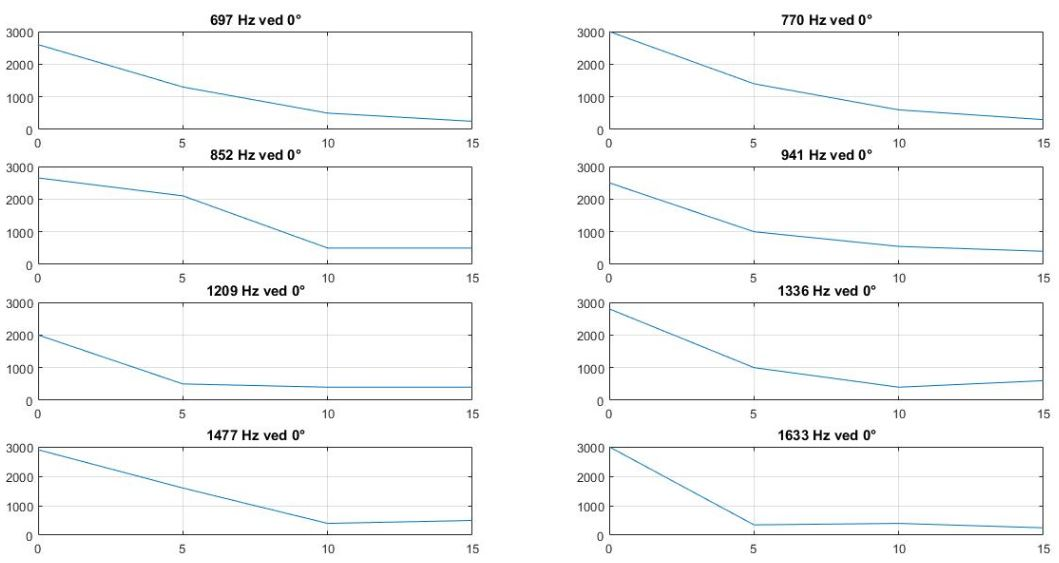
\includegraphics[scale=0.5]{Billeder/0degrees.jpg}
\caption{Langs y-aksen kan man se den gennemsnitligt højeste magnitude for et signal. Samme signal er blevet målt ved forskellige afstande som er plottet ud ad x-aksen}
\label{fig:degrees}
\end{figure} 

\subsection{Vinduefunktioner} \label{sec:Windowfunction}

Når et signal samples, kan der opstå spectral leakage, hvis signalet er ude af fase, når man kommer til sidste sample. Denne diskontinuitet (figur \ref{fig:Spectral})\footnote{Digital Signal Processing, kapitel 4.3} tilfører støj til signalet i form a frekvenser, der egentlig ikke er til stede. Man kan blandt andet mindske indflydelsen af spectral leakage ved at gange en såkaldt vinduefunktion på alle samples. Vinduet går mod 0 i enderne, og er højest midt i signalet.\\
Spectral leakage vil nødvendigvis blive et problem, når der vælges en fast mængde af samples, der kigges på til at finde forskellige frekvenser. Det skal derfor også undersøges om problemet er stort nok til at det er nødvendigt at gøre noget ved det - der skal helst ikke foretages for mange beregninger i goertzel-algoritmen, da den bliver brugt hele tiden. For at teste det kan man plotte magnitude for det samme signal, med forskellige vinduer ganget på. 

\begin{figure}[h!]
\centering
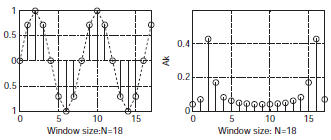
\includegraphics[scale=0.8]{Billeder/SpectralLeak.PNG}
\caption{Her kan man se at der kommer uønskede frekvenser med i signalet, fordi N er valgt så samplingen stopper et stykke inde i 3. periode}
\label{fig:Spectral}
\end{figure} 



\begin{figure}[h!]
\centering
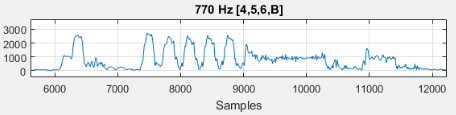
\includegraphics[scale=0.8]{Billeder/NoWindow.PNG}
\caption{Her ses magnitude på 770 Hz for et signal sendt med en tonelængde på 20 ms, uden en vinduefunktion på modtagersiden}
\label{fig:NoWindow}
\end{figure}

\begin{figure}[h!]
\centering
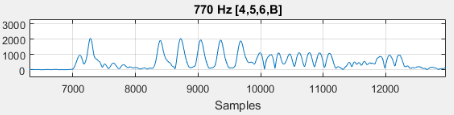
\includegraphics[scale=0.8]{Billeder/HannWindow.PNG}
\caption{Her ses magnitude på 770 Hz for samme signal sendt med en tonelængde på 20 ms, med et Hann-vindue på modtagersiden}
\label{fig:HannWindow}
\end{figure}

Signalet på figur \ref{fig:NoWindow} og \ref{fig:HannWindow} indeholder fem toner, hvor 770 Hz indgår. De steder hvor magnitude stiger til godt 50 \% af de store peaks, er der toner, hvor 697 Hz indgår. Det gør margenen, hvor man kan placere grænseværdien ret smal - det er et problem der bliver værre jo kortere toner man sender (se \ref{sec:hastighedstest}). Typen af vinduefunktion gør ikke den store forskel, men forskellen fra at køre med og uden er ret markant. Man kan opleve spikes, hvor magnitude stiger op på et niveau, der ligger meget tæt på grænseværdien (se figur \ref{fig:NoWindow} ved sample 9000). Det kan derfor konkluderes at det er nødvendigt at bruge en vinduefunktion, hvis man er interesseret i at sende korte toner.

\subsection{Hastighedstests} \label{sec:hastighedstest}

For at afgøre hvilken indflydelse tonebredden har på, hvor svært det er at afkode de rigtige frekvenser, kigges der igen på magnitudes for det samme signal, men her ved forskellige tonebredder. En af effekterne ved at forkorte tonelængden er at alle frekvens-bins bliver bredere, fordi antallet af samples man kigger på ad gangen bliver mindre - det betyder at frekvensopløsningen også falder, og det kan have den effekt at frekvenser, der ligger tæt på hinanden kan komme til at ligge i samme bin eller meget tæt på hinanden. 

\begin{figure}[h!]
\centering
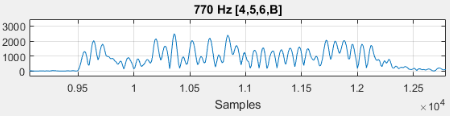
\includegraphics[scale=0.8]{Billeder/Speed10ms.PNG}
\caption{770 Hz 10 ms}
\label{fig:10ms}
\end{figure} 

\begin{figure}[h!]
\centering
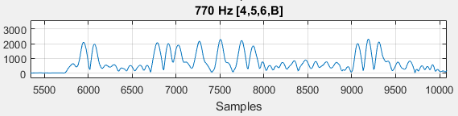
\includegraphics[scale=0.8]{Billeder/Speed15ms.PNG}
\caption{770 Hz 15 ms}
\label{fig:15ms}
\end{figure} 

\begin{figure}[h!]
\centering
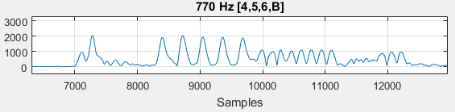
\includegraphics[scale=0.8]{Billeder/Speed20ms.PNG}
\caption{770 Hz 20 ms}
\label{fig:20ms}
\end{figure} 

\begin{figure}[h!]
\centering
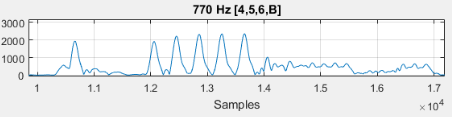
\includegraphics[scale=0.8]{Billeder/Speed25ms.PNG}
\caption{770 Hz 25 ms}
\label{fig:25ms}
\end{figure} 

\begin{figure}[h!]
\centering
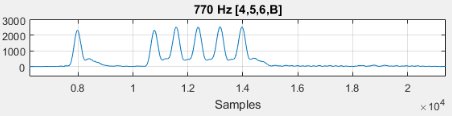
\includegraphics[scale=0.8]{Billeder/Speed50ms.PNG}
\caption{770 Hz 50 ms}
\label{fig:50ms}
\end{figure} 

Rent visuelt bliver det svært at afkode nogen information, ved tonebredder under 20 ms, og selv ved 20 ms er margenen for placeringen af grænseværdien ret smal. Ved de nuværende forhold er 25 ms, nok det mest stabile, men 20 ms kan også lade sig gøre, hvis man får lavet sig en fornuftig grænseværdi.

Something something zero-padding... Det kan muligvis lade sig gøre at øge frekvensopløsning ved at zero-padde de samples, der bliver behandlet i goertzel-algoritmen.

\subsection{DTMF-tone transition} \label{sec:ToneTransition}

Til at hjælpe med synkroniseringen moduleres signalet på afsendersiden, så amplituden er størst i midten af tonen og går mod 0 i enderne. Det har også den effekt at signalet ikke lige pludselig hopper tilbage til 0, når der skiftes til en ny tone, hvis signalet ikke er i fase i overgangen. Det får højtalerne til at poppe og bidrager med unødig støj til signalet. Oprindeligt blev der kun moduleret så amplituden steg lineært fra 0 \% i starten af tonen til 100 \% i midten og derfra faldt den lineært til 0 igen (se figur \ref{fig:modulation}). 

\begin{figure}[h!]
\centering
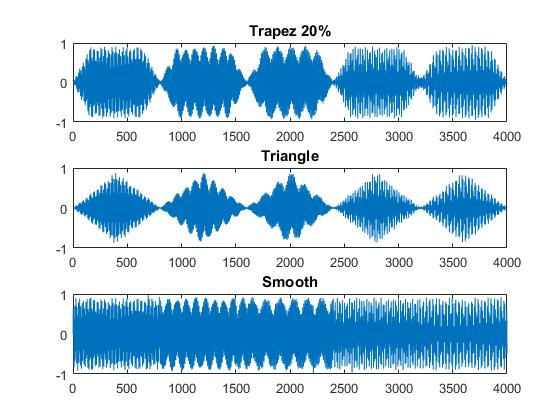
\includegraphics[scale=0.6]{Billeder/Modulation.PNG}
\caption{Her ses de forskellige modulationer, der blev anvendt}
\label{fig:modulation}
\end{figure} 

Moduleringen betyder at man skærer en masse af et ellers fint signal fra. Derfor var det smart at teste om man kunne få bedre resultater ved at modulere lidt anderledes, og så holde det op imod et signal uden modulation. Der blev forsøgt med en funktion der modulerede en trapez ovenpå signalet, så signalet blev holdt på 100 \% amplitude i længere tid (se figur \ref{fig:modulation}), og en funktion der tvinger fasen i 0 lidt blødere end, hvis der ikke havde været nogen modulation. 

\begin{figure}[h!]
\centering
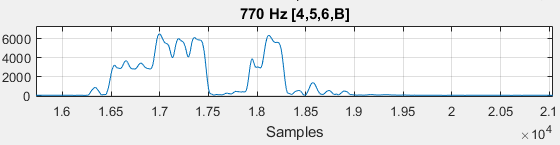
\includegraphics[scale=0.8]{Billeder/Snap.PNG}
\caption{Her ses et signal uden modulation}
\label{fig:snap}
\end{figure} 

\begin{figure}[h!]
\centering
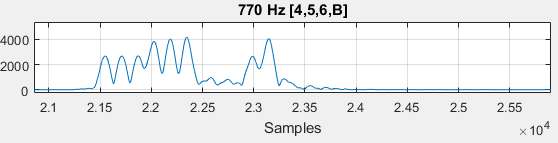
\includegraphics[scale=0.8]{Billeder/Triangle.PNG}
\caption{Her ses trekant-signalet}
\label{fig:triangle}
\end{figure} 

\begin{figure}[h!]
\centering
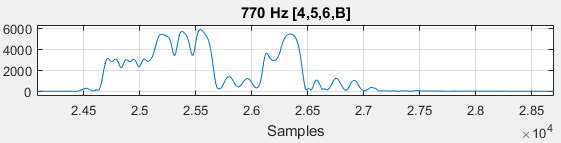
\includegraphics[scale=0.8]{Billeder/Steep10.PNG}
\caption{Her ses trapez-signalet}
\label{fig:steep10}
\end{figure} 

\begin{figure}[h!]
\centering
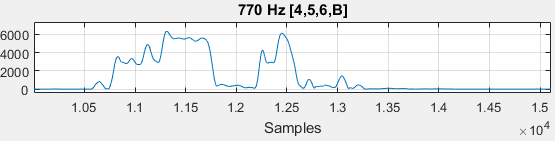
\includegraphics[scale=0.8]{Billeder/Smooth.PNG}
\caption{Her er signalet hvor fasen tvinges i 0}
\label{fig:smooth}
\end{figure} 

Det kan ses at magnitude for de to nye moduleringer (se figur \ref{fig:steep10} og \ref{fig:smooth}) er større og til stede i længere tid. Men ingen af dem er mærkbart bedre eller værre, end hvis der ikke er nogen modulering. Magnitude er mindre på trekant-signalet, men alle peaks er bedre definerede og der er ikke så meget støj.